
\documentclass{frontiersSCNS} % for Science articles

\usepackage{url,lineno}
%\linenumbers

%----------------------------------------------------------------------
% Own stuff
\usepackage{ucs}
\usepackage[utf8x]{inputenc}
\usepackage{xspace}
\usepackage{textcomp}
\newcommand{\permil}{\,\textperthousand\xspace}
\newcommand{\tbw}[1]{{\bf\parindent0pt\color{red}#1}}
\usepackage{minted}
\newminted{python}{showspaces=false,
  showtabs=false,
%  linenos=true,
  fontsize=\tiny,
  mathescape=true,
  frame=leftline,
  framerule=0pt,
  framesep=0mm}
%----------------------------------------------------------------------

\copyrightyear{}
\pubyear{}

\def\journal{Neuroinformatics}%%% write here for which journal %%%
\def\DOI{}
\def\articleType{Research Article}
\def\keyFont{\fontsize{8}{11}\helveticabold }
\def\firstAuthorLast{Djurfeldt {et~al.}}
\def\Authors{Mikael Djurfeldt\,$^{1,2,*}$, Andrew P. Davison\,$^{3}$,
 and Jochen M. Eppler\,$^4$}
% Affiliations should be keyed to the author's name with superscript
% numbers and be listed as follows: Laboratory, Institute, Department,
% Organization, City, State abbreviation (USA, Canada, Australia), and
% Country (without detailed address information such as city zip codes
% or street names).  If one of the authors has a change of address,
% list the new address below the correspondence details using a
% superscript symbol and use the same symbol to indicate the author in
% the author list.
\def\Address{$^{1}$PDC Center for High-Performance Computing, KTH
  Royal Institute of Technology, Stockholm, Sweden\\
  $^{2}$International Neuroinformatics Coordinating Facility (INCF),
  Stockholm, Sweden\\
  $^{3}$Unité de Neurosciences, Information et Complexité (UNIC),
  CNRS, Gif sur Yvette, France\\
  $^{4}$Institute of Neuroscience and Medicine (INM-6) and Institute
  for Advanced Simulation (IAS-6), Jülich Research Centre and
  JARA, Jülich, Germany}
% The Corresponding Author should be marked with an asterisk Provide
% the exact contact address (this time including street name and city
% zip code) and email of the corresponding author
\def\corrAuthor{Mikael Djurfeldt} \def\corrAddress{International
  Neuroinformatics Coordinating Facility (INCF), Nobels väg 15 A,
  Stockholm, SE-17177, Sweden} \def\corrEmail{djurfeldt@incf.org}

% \color{FrontiersColor} Is the color used in the Journal name, in the
% title, and the names of the sections

\begin{document}
\onecolumn
\firstpage{1}

\title[CSA in NEST and PyNN]{Modeling connectivity: Connection-set
 Algebra in NEST and PyNN}
\author[\firstAuthorLast ]{\Authors}
\address{}
\correspondance{}
\extraAuth{}% If there are more than 1 additional author, comment this
%line and uncomment the next one
%\extraAuth{corresponding Author2 \\ Laboratory X2, Institute X2,
%Department X2, Organization X2, Street X2, City X2 , State XX2 (only
%USA, Canada and Australia), Zip Code2, X2 Country X2,
%email2@uni2.edu}
\topic{Python in Neuroscience II}

\maketitle
\begin{abstract} % maximum 2000 characters including spaces

Most neuronal network simulators provide simulator-specific methods
for specifying connectivity. Thus, modelers need to learn the ways of
each simulator and connectivity descriptions are not easily moved
between them.  To improve this situation, several universal
description languages for neuronal network models (e.g. PyNN, NeuroML
and NineML) have been developed.

There is commonly a choice between explicitly specifying individual
connections or selecting one of a predefined set of connection
primitives. Such primitives are usually well suited for building
random balanced networks, synfire chains and recurrent networks
without much structure, however they often either lack the required
expressiveness or their implementations lack the required
computational efficiency to specify the connectivity of complex
hierarchical network models.

The connection-set algebra is a formalism for specifying the
connectivity of neuronal network models. CSA provides operators to
combine simpler connectivities into more complex ones and also
provides parameterization of such sets. The CSA is expressive enough
to describe a wide range of connectivities and can serve as a concise
notation for network structure in scientific writing as well as in
model description code for neural simulations. CSA implementations
allow for scalable and efficient representation of connectivity in
parallel neuronal network simulators.

Here, we describe the use of CSA and how it is coupled to the neural
simulation tool NEST through the new \verb|ConnectionGenerator|
interface provided by the \verb|libneurosim| library. We demonstrate
how CSA can be used for the specification of connectivity in the
simulator-independent neural specification language PyNN and how using
CSA as a high-level representation of connectivity patterns avoids
performance penalties and results in good scalability when transferred
to the simulator.

\tiny
 \keyFont{ \section{Keywords:} model description, connectivity,
 neural simulation, Python, large-scale modeling } %All article
 %types: you may provide up to 8 keywords; at least 5 are mandatory.
\end{abstract}

\section{Introduction}

The current trend towards neuronal network models which integrate
layers, columns and areas, brings with it the need for describing the
associated complex connectivity patterns. Currently, most simulators
use their own methods for describing connections between neurons. This
requires users to learn the ways of each simulator. Furthermore it
makes it hard to port models from one simulator to another and leaves
the efficient implementation of connection-generating functions as a
task for simulator developers. Especially in a parallel environment,
this is not a trivial undertaking. One way to ease this problem is the
use of general connection-generating libraries like the Connection-set
Algebra \citep[CSA;][]{djurfeldt12} or the graph library developed for
NineML \citep{raikov10}. They allow simulator-independent
specification of connectivity and enable high-level descriptions which
can be passed to a simulator core for efficient, parallelized, setup
of connectivity, avoiding the overhead associated with scripted
algorithms.

To take account of the fact that different users prefer different
simulators and also might prefer different libraries to create
connectivity, we created a generic \emph{connection generator}
interface. It enables the use of CSA and similar libraries in
different neuronal simulators. The interface makes both the simulator
and the connection-generating library replaceable and therefore gives
maximum flexibility to the user.

The remainder of this section will introduce related work and the
different components (CSA, PyNN, NEST) that were made to work with the
connection generator interface. The remaining sections will give a
short introduction to CSA, explain the interface itself and our
modifications and extensions to the components and the interplay
between them. We provide benchmark results that demonstrate the
excellent scaling of the implementation of the interface and close
with a discussion of the interface and an outlook to further
extensions.

\subsection{NeuroML and NineML}
NeuroML \citep{gleeson10,goddard01} is a declarative, XML-based, model
description language with a main focus on biologically detailed
models. It aims to describe the biophysics, anatomy and network
architecture of neuronal systems at multiple scales and to facilitate
the exchange of complex neuronal models between researchers. Although
NeuroML is, to the extent that XML allows, human readable it can also
be read and written by software tools such as
%XML editors,
graphical model construction environments \citep{gleeson07} and
neuronal simulators. The NetworkML layer of NeuroML allows for either
explicit lists of connections or implicit specification of connections
through selection from a limited palette of algorithms such as
all-to-all, one-to-one or different forms of random connectivity.
%Thus, NeuroML can play the
%role of an interface, not only between researchers but also between
%software tools. This enables modularity and software re-use in the
%sense that model construction and simulation can be performed using
%different tools.

In 2008, the oversight committee for the INCF Multiscale Modeling
Program identified two needs which were not fulfilled by other
declarative neuronal network model description languages at the time:
1. unambiguous specification of arbitrary models of synapse and neuron
dynamics, 2. specification of arbitrary network layout and
connectivity algorithms.  A task force was assembled to develop the
declarative, XML-based language NineML \citep{raikov11} which had an
initial focus on spiking neuronal network models with
integrate-and-fire dynamics.  One of the innovations was the division
of the language into a user layer (UL), corresponding to the level of
specification used in NeuroML, and an abstraction layer (AL),
providing the ability to unambiguously give definitions of the
concepts used in the UL. The UL defines the syntax for supplying
parameter values to abstract connectivity patterns. In the NineML DAE
tools \citep{nikolic10} prototype implementation, such patterns can be
defined in the AL using connection-set algebra, but the framework
allows for alternative XML-based connectivity descriptions.

This work inspired similar developments in NeuroML resulting in LEMS,
an XML-based language corresponding to the level of specification used
in the NineML AL.  Methods for declarative specification of
connectivity-patterns in LEMS are under development.  For example, the
all-to-all pattern can be defined using the \verb|ForEach| construct.

\subsection{CSA}
The connection-set algebra \citep[CSA;][]{djurfeldt12} is a formalism
for network connectivity which can be used both when describing a
network to a fellow researcher and when implementing a model for a
simulator.  It is currently focused on connectivity which has a
constructive or statistical element such that it can be specified by
an algorithm but it can also be used when all network connections are
given or in cases where only some elements of the connectivity are
explicitly specified. The distinguishing aspects of CSA are:
\begin{itemize}
\item It is abstract. CSA deals with sets of \emph{connections}. A
  connection is basically just an edge in a graph, with associated
  parameters. There is a clean separation between CSA and other
  aspects of model or simulator infrastructure.
\item A connection-set can represent a \emph{type} of
  connectivity---a connectivity pattern---in addition to the connectivity
  of a specific network.
\item It is an algebra: There are pre-existing connection-sets and
  operators to define new connection-sets in terms of existing.
\item It enables a succinct and precise description and definition of
  connectivity in terms of such algebraic expressions.
\item There are ways to implement CSA on a computer which are both
  efficient and scalable on a parallel computer.
\end{itemize}
There exist multiple implementations of CSA (see section
\ref{sec:impl}).

\subsection{PyNN}\label{sec:pynn}

PyNN \citep[\url{http://www.neuralensemble.org/PyNN};][]{Davison09} is
a community driven effort to provide a simulator-independent API for
describing neuronal networks in Python. Given a PyNN/Python model
description, the user can choose which simulator to use without a need
for changes to the model script. This is achieved through a set of
\emph{simulator backends} which may be part of the PyNN code base or
distributed separately. A backend adapts PyNN to a specific simulator.

In PyNN, a neuronal network is built from \verb|Population|s of
neurons and \verb|Projection|s between them. Each \verb|Projection| is
created by a \verb|Connector|, which knows how to set up the individual
connections. Different \verb|Connector|s exist and allow to set up a variety
of different connection patterns.

However, one of the regular problems with this approach is that PyNN
needs to break up the compact high-level description of connectivity
given by users into the commands understood by the respective
backend. These are often already too low-level (e.g. convergent or
divergent connects, one-to-one connects) and thus entail a certain
performance penalty due to data transfer and function call overhead.

The problem of excessive data transfers between PyNN and the simulator
can be solved by passing a high-level description of connectivity to
the simulator. This representation can be iterated and expanded at the
simulator level and thus avoid overhead. Moreover, this allows
efficient parallelization at the lower software layers.  The design of
a new \verb|Connector| for the NEST backend that implements this
solution is explained in section \ref{sec:conn_gen_pynn}. Section
\ref{sec:benchmarks} contains runtime and scalability benchmarks for
the new connector.

\subsection{NEST}

NEST is a simulator for large networks of point neurons or neuron
models with few electrical compartments
\citep[\url{http://www.nest-initiative.org};][]{Gewaltig_07_11204}. It
is suited for a broad range of neuronal network modeling approaches
and runs on a large variety of computer architectures. NEST is
parallelized using OpenMP \citep{OpenMPSpec} and MPI
\citep{MPIForum94} and scales well on large clusters of multi-core
processors and supercomputers \citep{Helias12_26}.

The network description is a script, written either in SLI, NEST's
built-in simulation language, or in Python, using the Python interface
to NEST \citep[PyNEST;][]{Eppler09_12}. The following description uses
the PyNEST syntax if not noted otherwise. To build a network in NEST,
the user first creates the neurons of the network and devices for
stimulation and measurement using the \verb|Create()| function and
then connects the elements with each other. NEST provides two basic
ways for creating connectivity.

\subsubsection*{Native connection functions:}

The most basic connect function, \verb|Connect()|, takes a list of
pre-synaptic neurons (or devices) and a list of the same amount of
post-synaptic neurons (or devices) and connects them in a one-to-one
fashion. Because of the function call overhead, this function is not
very efficient to use when creating large networks.

For such cases, the connection functions \verb|ConvergentConnect()|
and \verb|DivergentConnect()| can be used to create multiple
connections with a single call. In addition, random variants for both
functions exist to support the user in creating networks on the basis
of knowledge of connectivity statistics. However, random connection
parameters (e.g. \emph{weight} or \emph{delay}) need to be drawn
manually by the user and supplied to NEST after the creation of
connections.

\subsubsection*{Topology module:}

To ease the creation of networks with topological relations between
the neurons and organizations of neurons into layers and areas, NEST
provides a Topology module \citep{Plesser_13}. It supports the user in
connecting neurons and randomly initializing synapse parameters based
on geometry or topological relationships in the network.

The design of the novel interface for using connection generators from
NEST is explained in section \ref{sec:conn_gen_nest}. In section
\ref{sec:benchmarks}, we provide benchmarks for different use case
scenarios of the interface. A comparison of the performance of the
novel CSA interface, the native connection routines and the Topology
module of NEST is subject to further work.

%----------------------------------------------------------------------

\section{The Connection-set Algebra}\label{sec:csa}

\subsection{Basic concepts}

In neuronal network simulations, we often want to specify a projection
between a source population of neurons $P_s$ to a target population
$P_t$.  A projection consists of many individual connections.  In
nature, one such connection corresponds to an axon forming a synaptic
contact on the spine/dendrite of a receiving neuron.  The basic
concept of a CSA connection-set is in the context of neuronal network
simulation defined as the set of connections between $P_s$ and $P_t$
along with zero or more per-connection parameters such as weight or
delay.

In order to create an abstraction barrier between the actual neurons
of a population $P$ and the CSA, we enumerate $P$ using non-negative
integers from an index set $\mathcal{I}$ and let a connection from
$P_s$ to $P_t$ be represented by the pair $(i, j)$, where $i \in
\mathcal{I}_s, j \in \mathcal{I}_t$.  Such indices are similar to
the GIDs (Global IDentifiers) of the NEURON and NEST simulators but
normally start at 0 and runs consecutively for each population.
Introducing this abstraction, in the form of a mapping from objects in
the simulation domain to integers, gives at least two major
advantages: 1. The CSA does not need to care about the nature of the
objects in $P$---they could just as well be synaptic boutons as neurons.
2. The index set $\mathcal{I}$ can be chosen to be infinite.  The
gain of this will be demonstrated in section \ref{sec:structure}.

\begin{figure}[ht]
\centering
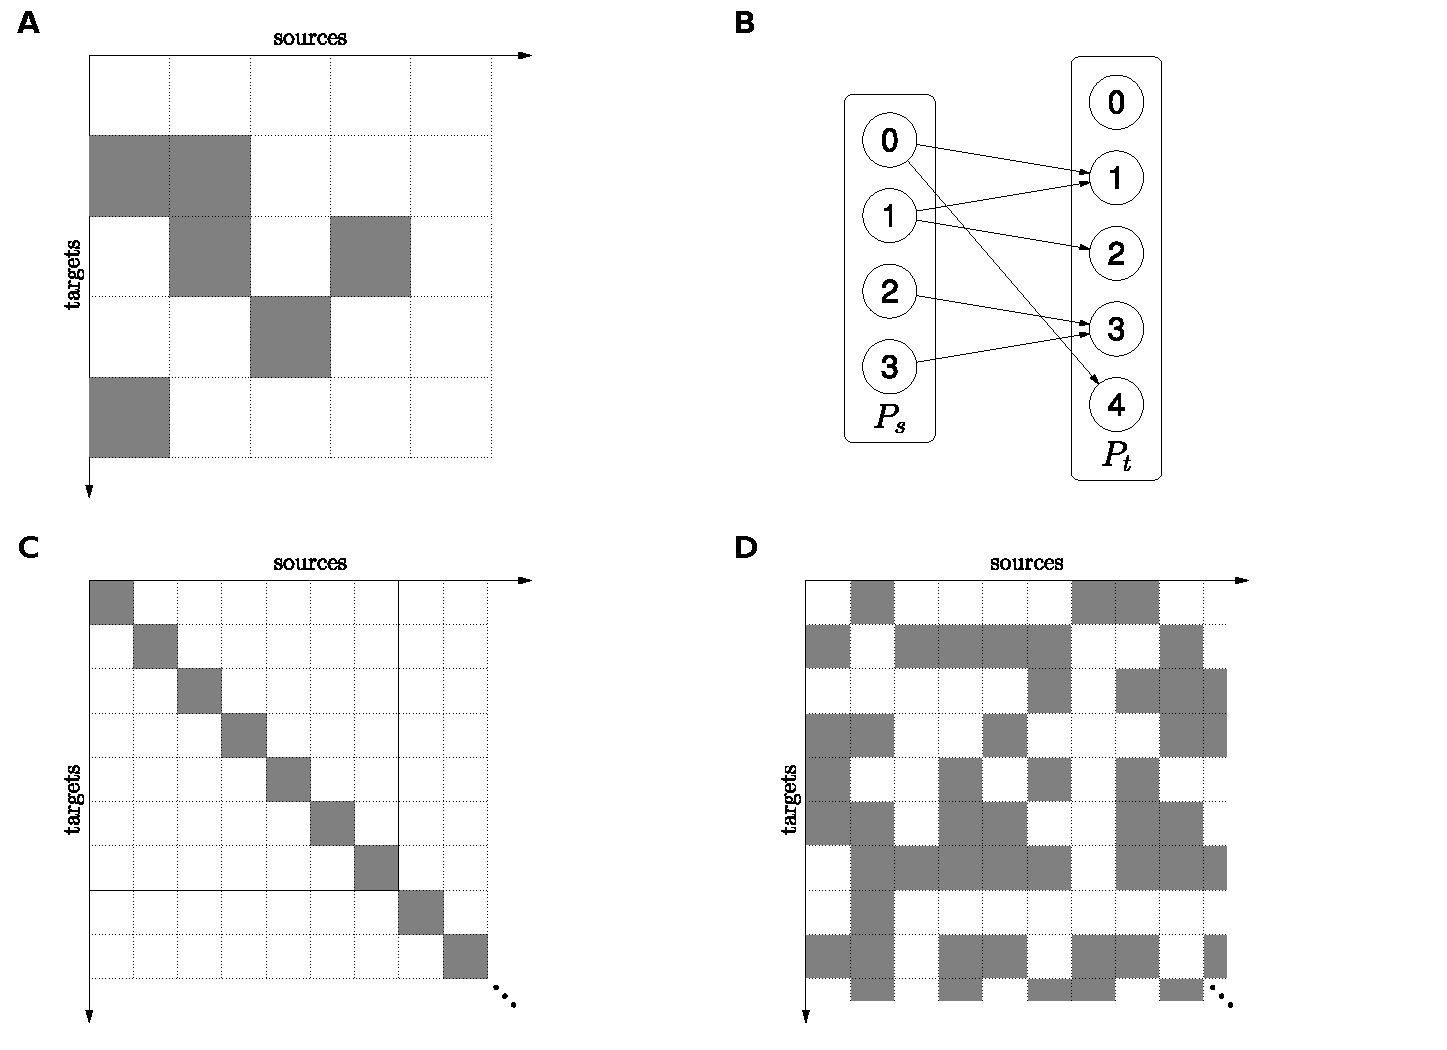
\includegraphics[scale=.7]{figures/csa-pane.pdf}
\caption{
  \textbf{A} The mask $\overline{M} =
  \{(0,1), (1,1), (1,2), (3,2), (2,3), (0,4)\}$ shown as a connection
  matrix. Grey squares represent existing connections.
  \textbf{B} Network connectivity when the mask in A is applied to
  source population $P_s$ and target population
  $P_t$.
  \textbf{C} The one-to-one mask $\bar{\delta}$. The mask is infinite,
  but finite portions can be cut out when applied to finite source and
  target populations. This is illustrated by the solid square for
  source and target size 7. When source and target population is the
  same, $\bar{\delta}$ represents self-connections.
  \textbf{D} The mask $\bar{\rho}(0.5) - \bar{\delta} =$ random
  connectivity without self-connections.
}\label{fig:csa} 
\end{figure}

A connection-set with zero parameters is called a \emph{mask}. A mask
tells which connections exist.  In the example of the mask
$\overline{M} = \{(0,1), (1,1), (1,2), (3,2), (2,3), (0,4)\}$ it can
be regarded either as a connection matrix (see Figure \ref{fig:csa}A)
or as a boolean indicator function:
\begin{equation}
\overline{M} : \mathcal{I}_s \times \mathcal{I}_t \rightarrow \{ \mathcal{F},
\mathcal{T} \}
\end{equation}
In the example $\overline{M}(0,0) = \mathcal{F}$ while
$\overline{M}(1,1) = \mathcal{T}$. If the mask is combined with a
source population $P_s$ and a target population $P_t$, the result is
the network $(P_s, P_t, \overline{M})$ shown in Figure \ref{fig:csa}B.

In CSA, connections can be parameterized through functions mapping
connections to values:
\begin{equation}
V : \mathcal{I}_s \times \mathcal{I}_t \rightarrow \mathcal{V}
\end{equation}
where $\mathcal{V}$ is some codomain. In the original CSA paper
\citep{djurfeldt12}, such a function is, somewhat inconsistently,
called a \emph{value set}. An example of a value set is distance
dependent delays with added noise sampled from a clipped random normal
distribution. Value sets are typically used to assign a weight or
delay to connections.

A CSA \emph{connection-set}, $C$, is a tuple of a mask and zero or
more value sets:
\begin{equation}
C = (\overline{M}, V_0, V_1, ...)
\end{equation}
The number of value sets of a connection-set is called its
\emph{arity}. A connection-set with arity 0 is for all purposes
equivalent to a mask and the two can be used interchangeably.

\subsection{An algebra for connectivity structure}\label{sec:structure}

In CSA, the basic concepts defined in the previous section have been
developed into a formalism for describing connectivity structure.
Assume that a mask is applied to a single population such that $P_s =
P_t = P$ and that we are interested in describing self-connections,
i.e. every neuron in $P$ should be connected to itself.  If the size
of $P$ is 4, the mask $\{(0, 0), (1, 1), (2, 2), (3, 3)\}$ could be
used.  If the size is 2, the mask $\{(0, 0), (1, 1)\}$ would be
appropriate. Such masks do not only contain information about
connectivity structure but also about population size. We can
generalize by stripping off the population size information and
allowing the index set $\mathcal{I}$ and mask to be infinite, defining
the one-to-one mask $\bar{\delta}$:
\begin{equation}
  \bar{\delta}(i, j) =
      \begin{cases}
        \mathcal{T}& \text{if $i = j$},\\
        \mathcal{F}& \text{otherwise}.
      \end{cases}
      \quad i, j \in \mathcal{I} = \mathbb{N}_0
\end{equation}
Now $\bar{\delta}$ only encapsulates the concept of self- or
one-to-one connectivity structure (depending on whether the source and
target population is the same or different), i.e. we can describe a
type of connectivity independently of any specific network.  Finite
portions can be cut out of such infinite connection-sets when applied
to finite populations (see Figure \ref{fig:csa}C).

CSA provides a set of elementary connection-sets such as
$\bar{\delta}$. Another example is the random mask $\bar{\rho}$, a
parameterized connection-set, or, more strictly, a mask-valued
function $\bar{\rho}(p)$ where the parameter $p$ is the probability
that a given connection $(i, j)$ exists.  That is, for each
combination of pre- and postsynaptic neurons, a Bernoulli trial
determines whether they are connected.
\begin{equation}
  \bar{\rho} (p) (i, j) =
  \begin{cases}
    \mathcal{T}& \text{with probability $p$},\\
    \mathcal{F}& \text{otherwise}.
  \end{cases}
  \quad i, j \in \mathbb{N}_0
\end{equation}
By using CSA \emph{operators} such as intersection, $\cap$, union,
$\cup$, and set difference, $-$, connection-sets can be combined into
expressions. For example, the idea of ``random Erd\H{o}s-R\'enyi
connectivity without self-connections'' can be represented by the CSA
expression $\bar{\rho}(p) - \bar{\delta}$ (see Figure
\ref{fig:csa}D). A mask representing all possible connections between
two finite populations can be formed by taking the Cartesian product
of their index sets, $\mathcal{I}_s \times
\mathcal{I}_t$. Intersecting with this mask can turn an infinite
connection-set, representing connectivity structure, into a connection
matrix between the populations. For example, the finite part of the
matrix in Figure \ref{fig:csa}C is $\{0..6\} \times \{0..6\} \cap
\bar{\delta}$. For a more in-depth description of the CSA and basic
principles of implementation, see \citet{djurfeldt12}.

%  \textbf{Figure 1.}{CSA Connection Matrix.}\label{fig:01}
%\subsection{Examples}
%  \textbf{Figure 2.}{An example of using CSA.}\label{fig:02}
%\subsection{Parallelization}
\subsection{Implementations}\label{sec:impl}

There currently exist three implementations of CSA.  The original
implementation is written in C++ and is part of the SPLIT simulation
library \citep{djurfeldt05}.  It was used to specify the connectivity
of the KTH cortex model \citep{djurfeldt08}---a model with three
hierarchical levels of structure.  The second implementation is
written in Python and is available as the Python library \verb|csa|.
Here, the purposes were 1. to get an easily usable and extensible
demonstration of CSA and 2. to experiment with new ways to implement
CSA. This implementation has been released as free software under the
GPL license and is available at the INCF software center
(\url{http://software.incf.org/software/csa}). A third implementation
in C++, \verb|libcsa|, is currently under development and will also be
released under the GPL license. It comes with Python bindings such
that CSA objects can be formed by Python level expressions with
similar syntax as used with the \verb|csa| library. For further
information about this syntax, the reader is referred to the tutorial
in the \verb|csa| package. The benchmarks in this article were
performed using the latter two implementations in Python and C++,
\verb|csa| and \verb|libcsa|.

% MDJ: I think I'll keep it like that. This paper is so complex
% conceptually anyway. We don't need to desribe everything!

%\subsubsection{Masks}
%\subsection{Python wrapper}
%\subsection{Serialization/deserialization}

%----------------------------------------------------------------------

\section{The Connection Generator API}

To allow users to flexibly choose among simulators and libraries which
generate connectivity, we developed an interface that abstracts the
simulator and the connection generating library from each other,
making both the simulator and the connectivity description library
replaceable.

\begin{figure}[ht]
\centering
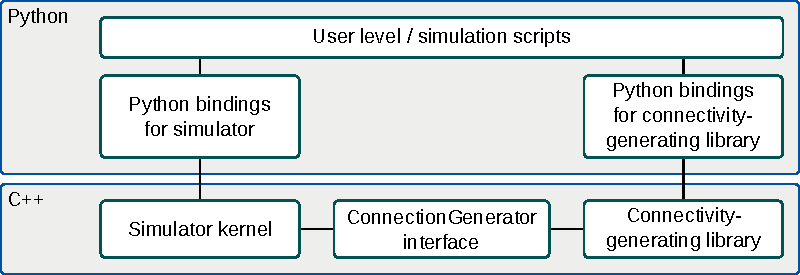
\includegraphics[scale=.8]{figures/block_diagram_conngen.pdf}
\caption{Block diagram of the connection generator interface and the
  components involved. The central component is the
  \texttt{ConnectionGenerator} class itself. It can connect to different
  simulators (e.g. NEST) and to different connection generating
  libraries (e.g. CSA). In this example, Python is used as scripting
  language for both simulator and connection generating
  library.}\label{fig:block_diagram_conngen}
\end{figure}

The basic idea is that a connection generating library, such as
\verb|csa| or \verb|libcsa| of section \ref{sec:impl}, is used to
create an object representing network connectivity.  In the case of a
CSA library, this object is a connection-set, but it could also be a
graph made through graph primitives. The \verb|ConnectionGenerator| interface
provides a C++ level interface to such objects which allows software
external to the connection generating library to efficiently iterate
through connections represented by the object.  In the example shown
in Figure \ref{fig:block_diagram_conngen}, the \verb|ConnectionGenerator|
interface is used to combine a Python scripted simulator with a Python
scripted connection generating library. A connection generating object
is assembled at the Python level.  If \verb|libcsa| is used, the
resulting object will be a C++ object with a Python wrapper. (See
lower two boxes to the right in the figure.) The object is used by a
C++ simulator kernel (lower box to the left) to specify network
connectivity. By providing connection generating software, with
Connection Generator API, as dynamically linked libraries, multiple
such libraries can be loaded into the Python runtime environment and
even used simultaneously without a need to recompile the simulator.

\subsection{The interface}\label{sec:cgint}

The interface is designed as an abstract base class in C++ and
consists of the following virtual functions:

\begin{unlist}
\item[\tt int arity()]: Return the number of per-connection values
  associated with this generator. Values can be parameters like
  weight, delay, time constants, or others.
\item[\tt int size()]: Return the number of connections represented by
  this generator.
\item[\tt void setMask(Mask\& mask)]: Inform the generator about which
  source and target indices are available. A
  \verb|ConnectionGenerator| mask represents the available nodes in
  the network for which to create connections.
\item[\tt void setMask(std::vector$<$Mask$>$\& masks, int local)]:
  This version of \texttt{setMask} is used by parallel simulators and
  informs the connection generator on the \verb|local| rank about the
  masks of all ranks. Different ranks usually have different masks
  since they are responsible for different subsets of the connections
  of the network. Some connection generators can use such information
  to avoid the need for communication with other ranks.
\item[\tt void start()]: Start an iteration. This function must be called
  before the first call to \verb|next()|.
\item[\tt bool next(int\& source, int\& target, double* value)]:
  Advance to the next connection or return false, if no more
  connections are available from the connection generator. Source and
  target indices of the connection as well as associated parameters
  are written into \verb|source|, \verb|target| and the array pointed
  to by \verb|value|, respectively. The order of iteration is
  according to increasing index, with all sources iterated over per
  target.
\end{unlist}

\subsection{libneurosim}\label{sec:libneurosim}
Where does the \verb|ConnectionGenerator| interface definition (in the
form of a C++ header file plus supporting code) belong?  If it is put
in the simulator or connection generating library source trees, it
will be duplicated over simulators or libraries.  As new versions of
the interface are developed, the situation will quickly become
unmanageable.  In fact, the \verb|ConnectionGenerator| interface is
unusual in that it is a symmetric abstraction barrier: it both allows
a given simulator to use any library supporting the API \emph{and}
allows the same library to be used from any simulator supporting the
API.

In order to create a space in which to put interfaces and other code
of generic use for neuronal network simulation software, we have
developed the neurosim library
(\url{http://software.incf.org/software/libneurosim}).  More
precisely, libneurosim is a software package which currently consists
of two main component libraries: \verb|libneurosim|, providing C++
level support code and \verb|libpyneurosim|, providing Python support
code.

\verb|Libneurosim| provides the \verb|ConnectionGenerator| interface
(Figure \ref{fig:block_diagram_conngen}, bottom). It also contains a
registry for XML parser functions.  Different types of connection
generators can be described by different XML-based languages.  For
example, the \verb|csa| library can serialize connection-set
expressions using a MathML-based language.  A connection generating
library may provide a parser for one or more such languages.
Conversely, the same XML-based language might be used by one or more
connection generating libraries.  The XML parser registry maps XML
tags identifying specific languages to specific connection libraries.
The interface to the registry consists of three static methods in the
\verb|ConnectionGenerator| interface:

\begin{unlist}
\item[\tt void selectCGImplementation (std::string tag, std::string
  library)]:\\ Associate the parent node tag \verb|tag| with the library
  \verb|library|.  The library named \verb|library| will be
  dynamically loaded and will invoke the \verb|libneurosim| function
  \verb|registerConnectionGeneratorLibrary| to register its XML
  parser.
\item[\tt ConnectionGenerator* fromXML (std::string xml)]: Parse the
  XML representation \verb|xml| of a connection generator and return
  it. The function dispatches to parsers of different libraries
  depending on previous calls to \verb|selectCGImplementation|.
\item[\tt ConnectionGenerator* fromXMLFile (std::string path)]: Same as
  previous function, but read the XML stream from the file with
  pathname \verb|path|.
\end{unlist}

\verb|libpyneurosim| currently contains generic support for
registering new Python connection generator types and unwrapping
instances of such objects:

\begin{unlist}
\item[\tt void registerConnectionGeneratorType (CheckFuncT,
  UnpackFuncT)]: Register a new type checking and unwrapping
  function.
\item[\tt isConnectionGenerator (PyObject* pObj)]: Check if
  \verb|pObj| is a known connection generator type (as identified by
  previously registered checking functions).
\item[\tt ConnectionGenerator* unpackConnectionGenerator (PyObject*
  pObj)]: Unwrap the connection generator in \verb|pObj| and return
  it.
\end{unlist}

\section{Using connection generators in NEST}\label{sec:conn_gen_nest}

To support the Connection Generator interface in NEST we created the
ConnectionGeneratorModule, a plugin for NEST which can be
(de-)activated at configure time. The module is built on top of
\verb|libneurosim| and extends both user interfaces (SLI and PyNEST)
with the following functions:

\begin{unlist}
\item[\tt CGConnect], which takes a connection generator \emph{cg},
  lists of GIDs for \emph{pre}- and a \emph{post}-synaptic
  populations, and a \emph{param\_map}. It creates the connections
  between neurons in \emph{pre}- and a \emph{post} as prescribed by
  the rules in \emph{cg}. The parameter map \emph{param\_map} maps
  parameter names (e.g. \emph{weight}, \emph{delay}) to their index
  for the parameter value vector created by the call to \verb|next()|
  in the \verb|ConnectionGenerator| interface (see section
  \ref{sec:cgint}).
\item[\tt CGParse], which takes a serialized version of a connection
  generator in the string \emph{xml} and returns the corresponding
  object. A special use of this function exists on supercomputers,
  where Python is often not available on the compute nodes, or where
  the memory and performance penalty would not be acceptable and a
  pure SLI-based solution is preferable.
\item[\tt CGParseFile], which takes a file name \emph{fname} and parses
  the serialized version of a connection generator contained therein.
\item[\tt CGSelectImplementation], which takes an XML tag \emph{tag}
  representing the parent node of a serialized connection generator
  and the name of a library \emph{library} to provide a parser for
  such an XML file. This information determines which library should
  carry out the parsing in for \verb|CGParse|.
\end{unlist}

When PyNEST is used, the connection generator can be created by the
user in Python using the Python wrapper of \verb|libcsa|. In the call
to \verb|CGConnect()|, a pointer to the underlying
\verb|ConnectionGenerator| object in C++ is converted into a SLI
Datum, which can be shipped into NEST's simulation kernel and handled
there using the C++ interface to the connection generator. In SLI,
there is no direct way of creating a connection generator. However,
the SLI function \verb|CGParse| can read a serialized version of a
connection generator from XML and reinstantiate the object, which can
then be given to SLI's version of the \verb|CGConnect| function.

\begin{figure}[ht]
\centering
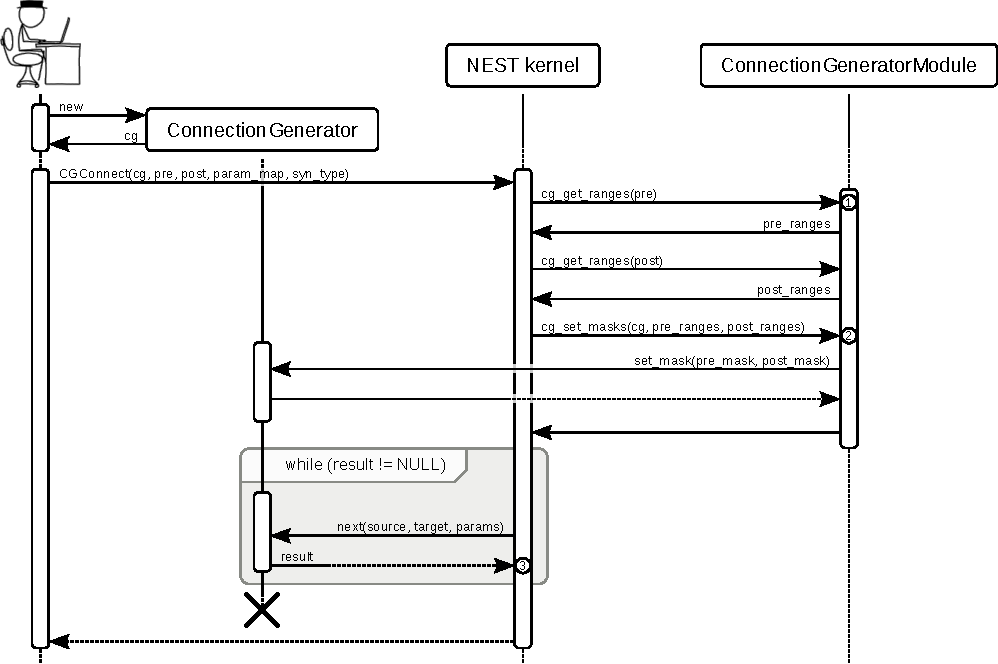
\includegraphics[scale=.8]{figures/sequence_diagram_nest.pdf}
\caption{Sequence diagram showing the function calls during the use of
  the \texttt{ConnectionGenerator} interface in NEST. The user first creates a
  \texttt{ConnectionGenerator} object \emph{cg}. She then calls
  PyNEST's \texttt{CGConnect()} function. \textcircled{\footnotesize
    1} The function \texttt{cg\_get\_ranges()} returns all contiguous
  ranges of global IDs (GIDs) in the given list as a vector of closed
  intervals, still using the GID representation.
  \textcircled{\footnotesize 2} At this point in time, the
  ConnectionGeneratorModule needs to translate the GIDs to CSA
  indices, which run from 0 and enumerate the elements of the given
  \emph{pre}- and \emph{post}-synaptic populations. The result of the
  translation (\emph{pre\_mask} and \emph{post\_mask}) is used to set
  the masks on \emph{cg}. \textcircled{\footnotesize 3} The NEST
  kernel iterates the connection generator by calling \texttt{next()}
  until there are no more connections. For each received connection,
  it creates the connection by calling \texttt{Network::connect()}. If
  a non-empty \emph{param\_map} was given to \texttt{CGConnect}, the
  connection's weight and delay are taken from the value-set in
  \emph{cg}.}\label{fig:sequence_diagram_nest}
\end{figure}

Figure \ref{fig:sequence_diagram_nest} shows the different entities in
NEST involved in a user call to \verb|CGConnect()|. After setting the
masks for the connection generator, the NEST kernel iteratively calls
\verb|next()| which returns the source and target index of the next
connection and parameter values for the connection. The connections
are established one by one by calling NEST's basic
\verb|Network::connect()| function.

A connection generator identifies nodes of the network using source
and target indices in ranges $[0, N_s-1]$ and $[0, N_t-1]$ where $N_s$
is the number of source neurons and $N_t$ the number of target
neurons, but NEST uses GIDs to identify neurons.  Internally,
\verb|CGConnect()| needs to maintain a mapping between connection
generator indices and GIDs.  Appendix A describes two aspects of this
mapping, the detection of contiguous ranges in the lists of GIDs
passed as arguments to \verb|CGConnect()| and index translation.

%----------------------------------------------------------------------

\section{Using connection generators in PyNN}\label{sec:conn_gen_pynn}

Since version 0.7, PyNN has provided the generic \verb|CSAConnector|, which can
iterate a CSA connection set and issue one by one connect calls to
the different backends. Internally, the connector executes the
following two steps:

\begin{enumerate}
\item Form a finite connection-set adapted to the actual sizes of the
  populations by intersecting the given connection set with the
  Cartesian product of the neuron indices of the pre- and
  post-synaptic populations.
\item Connect the neurons. The weight, delay and any other synaptic
  parameters are taken from the connection set, if supplied as value
  sets (see section \ref{sec:csa}), and from the parameterization of
  the synapse type otherwise.
\end{enumerate}

During this study, we extended the NEST backend for PyNN with a new
and specialized \verb|CSAConnector| which passes the complete
connection generator object down to the simulator (by calling PyNEST's
\verb|CGConnect()|). The iteration over the connections can then take
place in NEST (see section \ref{sec:conn_gen_nest}). This greatly
reduces the overhead and thus improves the runtime and scalability of
connection generation (section \ref{sec:benchmarks}).

%----------------------------------------------------------------------

\section{Benchmarks}\label{sec:benchmarks}

We ran a series of benchmarks in order to assess the performance of
and compare two implementations of CSA (see section \ref{sec:impl})
and the two implementations of the \verb|CSAConnector| for PyNN (see section
\ref{sec:conn_gen_pynn}). Grouped by the software layer on which the
iteration of the connection generator happens (either in Python by PyNN
or in C++ by NEST) and the CSA implementation used (\verb|csa| is the Python
version, \verb|libcsa| the C++ version), the following scenarios were
measured:

\begin{itemize}
\item \textbf{Python, csa} used PyNN's original \verb|CSAConnector|
  that is available for all backends in combination with the Python
  CSA implementation. The \verb|CSAConnector| intersects the
  \verb|csa| object with a mask representing the actual source and
  target nodes available and iterates the \verb|csa| object entirely
  at the Python level. It connects the neurons by issuing
  \verb|ConvergentConnect()| calls to PyNEST.
\item \textbf{C++, csa} used the new \verb|CSAConnector| for PyNN's NEST
  backend, which is available in the development version of PyNN, and the
  Python CSA implementation. The \verb|csa| object is passed down to NEST
  through \verb|CGConnect()|. The ConnectionGeneratorModule then
  iterates it at the C++ level by repeatedly calling the Python level
  iterator.
\item \textbf{Python, libcsa} used the generic \verb|CSAConnector| in
  PyNN and the C++ CSA implementation \verb|libcsa|. The
  \verb|CSAConnector| iterates the \verb|libcsa| object at the Python
  level, repeatedly calling its C++ connection generator.
\item \textbf{C++, libcsa} used the new \verb|CSAConnector| for PyNN's
  NEST backend and the C++ CSA implementation \verb|libcsa|. The
  \verb|libcsa| object is passed down to NEST through
  \verb|CGConnect()|. All iteration happen in C++ in the
  ConnectionGeneratorModule.
\end{itemize}

\begin{figure}[ht]
\centering
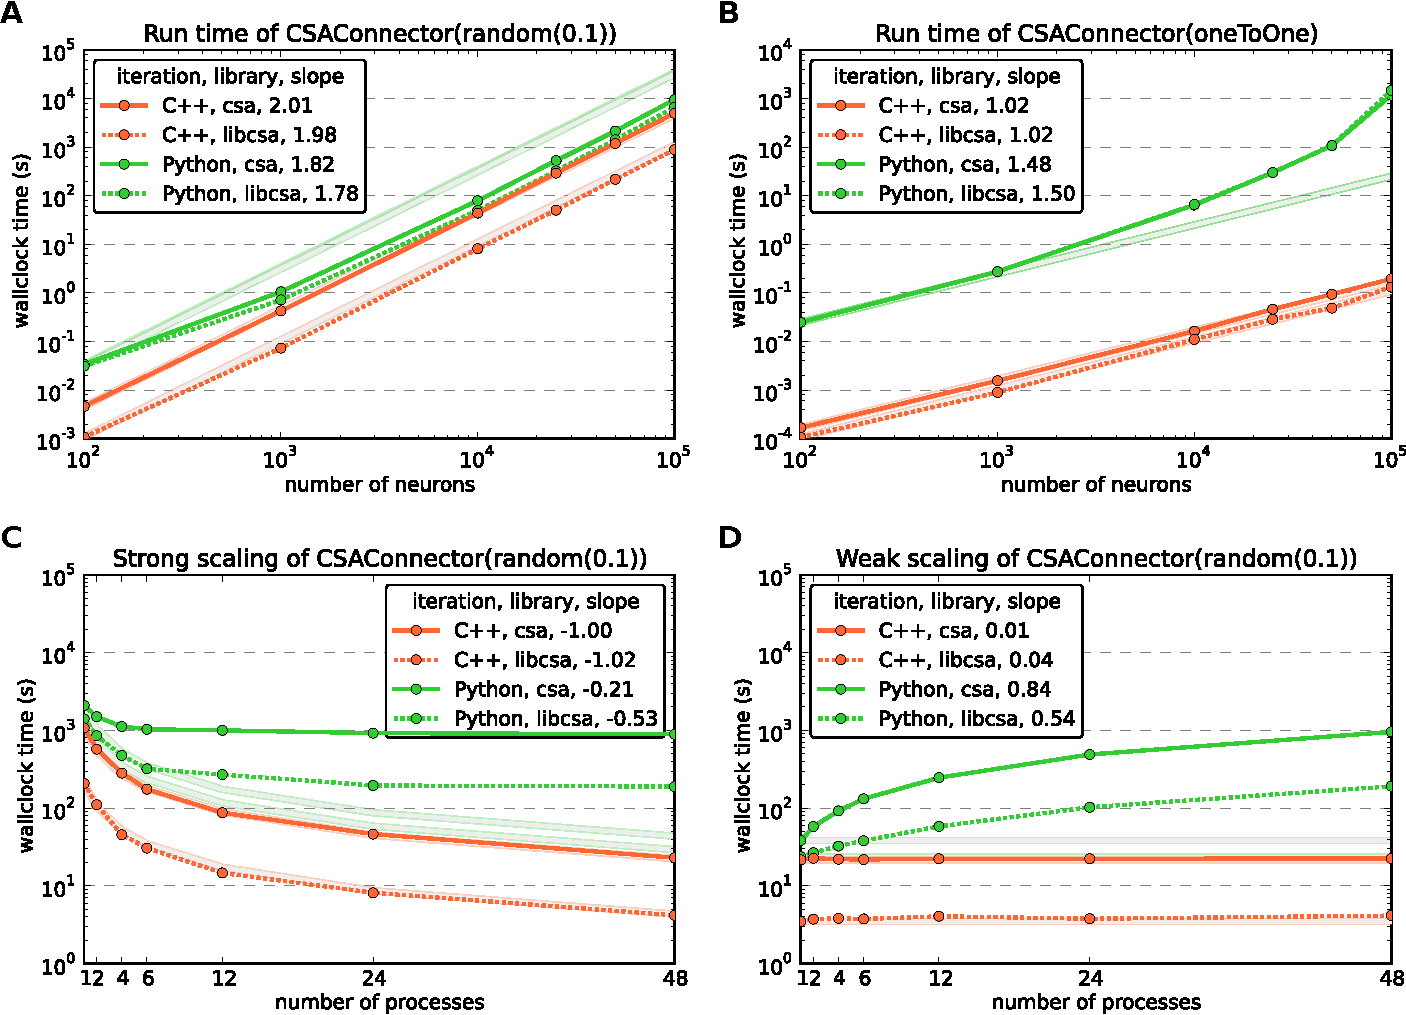
\includegraphics[scale=.7]{benchmarks/CSAConnector.pdf}
\caption{Benchmark results for the use of CSA in NEST through PyNN,
  comparing the two \texttt{CSAConnector} implementations explained in
  section \ref{sec:conn_gen_pynn} and the two CSA implementations
  mentioned in section \ref{sec:csa}. Color and dash codes are given
  in the legends. Slope is the ratio of logarithms of the last and
  first data point shown. Pale lines denote the expected
  scaling. \textbf{A} shows the run time for connecting a network
  using CSAs \emph{random} mask with a probability of 0.1 for
  different numbers of neurons. This connector creates $O(n^2)$
  connections for $n$ neurons. The expected slope is thus
  2. \textbf{B} shows the same as in A, but using CSAs \emph{oneToOne}
  mask, which creates $O(n)$ connections for $n$ neurons and has an
  expected slope of 1. \textbf{C} shows a strong scaling experiment,
  wiring a network of 48,000 neurons using CSAs \emph{random} mask
  with a probability of 0.1 and varying the number of MPI processes
  from 1 to 48. The expected slope is -1, meaning that the run time
  drops linearly with the number of processes. \textbf{D} shows the
  results of a weak scaling experiment, increasing the number of
  connections by approx. $4.8 \cdot 10^6$ per additional MPI process
  for 1 to 48 processes. The expected slope is 0, as the load
  increases linearly with the number of
  processes.}\label{fig:pynn_benchmarks}
\end{figure}

The population size benchmarks (figure \ref{fig:pynn_benchmarks}A and
B) used one MPI process and varied the number of neurons from $10^2$
to $10^5$ with one sample per order of magnitude. All tested
implementations of CSA (\verb|csa|, \verb|libcsa|) scale perfectly
with slopes around 2 for the \emph{random} mask, independently of the
software layer (C++ or Python), on which the iteration was carried
out. However, in Figure \ref{fig:pynn_benchmarks}, the vertical
offsets and the increasing slopes of the curves for the generic
\verb|CSAConnector| which iterates at the Python/PyNN level suggest
that the current implementation of this connector together with calls
through different software layers to setup individual connections adds
a significant overhead to the process of connection generation.

To demonstrate the scalability of the implementations, we carried out
both weak and strong scaling benchmarks, using CSA's \emph{random}
mask with a probability of $0.1$ (figure \ref{fig:pynn_benchmarks} C and
D). For each of them, the number of MPI processes was varied from 1 to
48.

In the strong scaling benchmark (figure \ref{fig:pynn_benchmarks}C),
the number of MPI processes was varied while keeping the total number
of neurons in the network fixed at $48000$. This resulted in
approx. 230 million connections created. It is easily visible that
iteration of the CSA object at the Python level in the current PyNN
implementation of the original \verb|CSAConnector| is detrimental to
the scalability. In contrast, it is possible to obtain perfect scaling
if the iteration of the CSA object is carried out from the C++
layer. Using the C++ implementation of CSA, it is, however, possible
to gain another order of magnitude compared to the Python version.

During the weak scaling benchmark (figure \ref{fig:pynn_benchmarks}C),
the number of MPI processes was varied while the work load was
increased by a fixed number of connections per additional process.
The number of connections grows quadratically with the number of
neurons when using CSA's \emph{random} mask with a fixed
probality. The number of neurons per process was thus increased with
the square root of the desired number of connections. In the realm of
natural numbers, this leads to a slight error, which was, however,
well acceptable with values between $-1.42$\permil and $+1.08$\permil.

The machine used for benchmarking was equipped with 4 12-core AMD
Operon 6174 (Magny Cours) processors organized into 8 NUMA domains
with 6 cores each. Other than the choice of the number of MPI
processes in a NUMA-friendly way, no measures (like pinning of
processes to cores, altering the affinity of threads to cores, etc.)
were taken to avoid distortions of the results.

%----------------------------------------------------------------------

\section{Discussion and outlook}

We have shown the design of a generic interface for coupling
connection generating libraries to neuronal simulators and
demonstrated good scaling when using it in NEST and PyNN. The
availability of this and associated interfaces lets users flexibly
choose a connection generating library independently of the simulator
used, and thereby grants greater freedom for describing models.

In the first version of the \verb|ConnectionGenerator| interface
presented here, emphasis was put on simplicity. There are several
possible directions of development. Currently, parameters are passed
as \verb|double|s. This could be generalized to other data types.  For
parallel simulators, connection generators may need access to the MPI
communicator.  Instead of using a fixed iteration order, the order
could be specified by the simulator. Iteration order could also be
unspecified, giving opportunities for more optimal iteration on the
part of the connection generating library.  In order to maintain
backward compatibility as new revisions of the interface is developed,
interface versioning could be introduced.

One limitation in the current implementations of the NEST
ConnectionGeneratorModule and the PyNN \verb|CSAConnector| is that value sets
for the connection generator can only be used if its arity is 0 or
2. This means that only values for weight and delay can be generated
by the connection generating library. For many synapse models it would
be beneficial to also set other parameters based on rules in the
connection generator. Examples of such synapse models are STDP or
short-term facilitation and depression.

If every single piece of generically useful functionality, such as the
\verb|ConnectionGenerator| interface, was distributed in a separate
library, the library dependencies of simulation software would grow
unmanageable.  Libneurosim could therefore become a place within which
to put other interfaces and supporting code besides the
\verb|ConnectionGenerator| interface. We are currently investigating
if the code for finding contiguous ranges and translating indices (see
Appendix A) can be extracted from NEST and made available as part of
\verb|libneurosim|.

Another possible extension could be code for the generation of random
numbers. The GNU Scientific Library (GSL;
\url{http://www.gnu.org/software/gsl}) provides random number
generators, but there are still needs specific to neuronal network
simulators which could be served by a specialized RNG library. Should
such a library be provided through the libneurosim software package?
We believe that the answer to this and similar questions is a matter
of judgement. It would certainly not make sense to collect all
generically useful functionality in one monolithic library.

%----------------------------------------------------------------------

\section*{Conflict-of-Interest Statement}
The authors declare that the research was conducted in the absence of
any commercial or financial relationships that could be construed as a
potential conflict of interest.

\section*{Acknowledgement}
This work was partially done under the INCF Multiscale Modeling
Program. It is partially supported by the Helmholtz Association: HASB
and portfolio theme SMHB, the Jülich Aachen Research Alliance (JARA),
the VSR computation time grant JINB33 on the JUQUEEN supercomputer in
Jülich, and EU Grant 269921 (BrainScaleS). The authors would like to
thank Randall Munroe of \url{http://www.xkcd.org} for granting the
permission to use one of his drawings in
Figure~\ref{fig:sequence_diagram_nest}.

\section*{Appendix A: Creating masks in NEST}\label{sec:creating_masks}

\subsection*{Identifying contiguous ranges}

All elements (neurons or devices) in NEST are identified uniquely by
an integer number, their global id (\emph{GID}). All connection
routines work either on single GIDs or on lists of GIDs. When calling
\verb|CGConnect|, the user supplies two a sorted lists of neurons as
pre- and post-synaptic populations. These lists do not necessarily
have to contain contiguous GIDs.

The contiguous ranges inside the given lists are found using a binary
search approach, where the left border of a range is always one past
the end of the last range and the right border is searched for. The
following listing contains the procedure to find all contiguous ranges
in a sorted list \emph{ls} as a Python script.

First, we initialize \emph{ranges} to an empty list, the left border
(\emph{left}) to 0, and \emph{end} to the last index of \emph{ls}.

\begin{pythoncode}
ranges = []
left = 0
end = len(ls) - 1
\end{pythoncode}

The following loop will terminate the search when the \emph{end} of
\emph{ls} is reached. Until this happens, it always finds the next
right border using \emph{get\_right()} and adds the range between
\emph{left} and \emph{right} to \emph{ranges}. If a new range is
found, left is set to one past the end of the last found range.

\begin{pythoncode}
while True:
    right = get_right(left, (len(ls) - left) / 2)
    ranges.append((ls[left], ls[right]))
    if right == end:
        break
    else:
        left = right + 1
\end{pythoncode}

The task of the \emph{get\_right()} function is to calculate and
return the right border of the contiguous range of GIDs in \emph{ls}
starting at \emph{left}. The element is found using a binary search
with stepsize \emph{step}. First, we check if \emph{left} is already
the index of the last element in \emph{ls}. If this is the case, we
return \emph{left} as the right border.

\begin{pythoncode}
def get_right(left, step):
    if left == end:
        return left
\end{pythoncode}

If there are numbers left to be considered, we set \emph{leftmost\_r},
the leftmost right border touched during the search, to \emph{None} to
mark it as unitialized. We then initialize the search index \emph{i}
to the last valid index into \emph{ls}, and \emph{last\_i} to \emph{i}.

\begin{pythoncode}
    leftmost_r = None
    i = last_i = end
\end{pythoncode}

In the following loop, we perform the search. If \emph{i} points to
the end of \emph{ls} and the distance between \emph{i} and \emph{left}
is the same as between the values \emph{ls[i]} and \emph{ls[left]}
(i.e. \emph{ls[i+1]} equals \emph{ls[i]+1} for all \emph{i}), or if
\emph{i} is pointing at the position of the leftmost right border we
found until now (i.e. we're back at an already visited index), we
found the right border of the contiguous range (\emph{last\_i}) and
return it.

\begin{pythoncode}
    while True:
        match = ls[i] - ls[left] == i - left
        if (i == end and match) or i == leftmost_r:
            return last_i
\end{pythoncode}

We now store the current value of \emph{i} in \emph{last\_i}. This is
the current candidate for the right border.

\begin{pythoncode}
        last_i = i 
\end{pythoncode}

If the range between \emph{ls[left]} and \emph{ls[i]} is contiguous, we
set \emph{i} to the right by \emph{step} steps, else update the
variable \emph{leftmost\_r} to the current \emph{i} (i.e. the known
leftmost position) and set \emph{i} to the left by \emph{step} steps.

\begin{pythoncode}
        if match:
            i += step
        else:
            leftmost_r = i
            i -= step
\end{pythoncode}

If we reach this point, we have to reduce the search interval
(\emph{step}) to half its size if it is still $>$ 1. This adaptation
is the basis of the binary search.

\begin{pythoncode}
        if step != 1:
            step /= 2
\end{pythoncode}

\subsection*{Index translation}

All elements in NEST are identified by their global id and thus the
range-finding procedure explained in the previous section returns the
ranges in the domain of GIDs. CSA however, expects neuron indices to
start at 0, i.e. it expects the indices into the pre- and
post-synaptic populations instead of the GIDs at that positions. This
means that we have to translate indices from NEST to CSA during the
setting of the masks and back when we actually create the connections.

As explained in section \ref{sec:csa}, the masks for the sources must
contain all local and remote nodes. The \emph{skip} of the mask is
therefore always set to 1. For the sources, the same source mask is
stored \emph{n\_proc} times on each process. The masks for the targets
must only contain the local nodes. This is achieved by i) setting
\emph{skip} to the number of MPI processes upon creation of the mask,
and ii) by taking the index-translated id of the first local neuron as
the first entry of the mask for that range. Together with the skip
this allows to find all local nodes in the range. If this
index-translation renders the resulting range empty (i.e. because the
first local id is beyond the last element of the range), the range is
not added to the mask.

\section*{Appendix B: Software versions used}

These benchmarks were using the development version of PyNN from 
https://github.com/NeuralEnsemble/PyNN/ (version db76c748cd) and NEST
revision XXXX from the internal Subversion repository.


\bibliographystyle{frontiersinSCNS&ENG}
\bibliography{pns2csa13}

\end{document}
